\section{Ejercicio 3}
\subsection{Problema}
Dise\~nar e implementar una \textbf{heur\'istica constructiva golosa} para List Coloring y desarrollar los siguientes puntos:\\

a) Explicar detalladamente el algoritmo implementado.\\

b) Calcular el orden de complejidad temporal de peor caso del algoritmo.\\

c) Describir instancias de List Coloring para las cuales la heur\'istica no proporciona una soluci\'on \'optima. Indicar qu\'e tan mala puede ser la soluci\'on obtenida respecto de la soluci\'on factible.\\

d) Realizar una experimentaci\'on que permita observar la performance del algoritmo en t\'erminos de tiempo de ejecuci\'on en funci\'on del tama\~no de entrada.\\
\subsection{Explicaci\'on y desarrollo del problema}


 A la hora de pensar una heruistica golosa, la mas simple y rapida podria ser pararse sobre un nodo al azar, elegir un color al azar y luego seguir con sus vecinos. Sin embargo esto podria generar muchisimos conflictos ya que depende estrictamente de la aleatoriedad con que elegimos los nodos y los colores. Lo que veremos a contiuacion, es que a esta herusitica recien mencionada se le pueden hacer pequenias mejoras tal que mejoren la performance del resultado.\\
 Empezaremos de un nodo al azar y recorreremos sus colores. Para cada uno de ellos iteraremos los vecinos del nodo en cuestion y preguntaremos si este vecino ya esta pintado y su color es el mismo en el cual estamos iterando. En este caso el color es invalido. En caso de que no este pintado, nos preguntaremos, si tiene mas de 1 color disponible y nuestro color en cuestion pertenece a la lista de colores de ese vecino, entonces tambien es invalido. En cualquier otro caso sera valido. Los casos donde puede ser valido es si el color en cuestion no se encuentra entre los colores disponibles del vecino en donde estamos iterando.\\ Ademas, puede suceder en un grafo poco feliz que nuestro nodo N tenga los colores 1,2,3 y que tenga 3 vecinos A,B,C cuyos unicos colores sean 1,2,3 respectivamente. En este caso decidimos que al salir del ciclo (es decir el ciclo no pudo decidir ningun color), pintamos al nodo N con el ultimo color de la lista. En este caso, por descarte, tambien sera un color valido.\\
 Luego de pintar el nodo, seguiremos iterando por los demas nodos.\\\\
 
 
 Esta heuristica tiene un defecto muy importante y puede comportarse muy mal en determinados casos.\\
 Imaginemos un grafo donde exista un coloreo valido, sin embargo para cada nodo, su color valido este en el final de la lista. Es posible que, par algun nodo, exista un color de la lista que sea valido localmente, sin embargo a gran escala no seria el correcto. Nuestro algoritmo recorre la lista de colores en orden, de manera tal que primero se encontraria con el color incorrecto, lo seteearia y el coloreo quedaria equivocado.
 
 La segunda heuristica pasa por exactamente el mismo proceso, salvo que a la hora de iterar los colores, no se queda con el primer color que es valido, sino que al encontrar un color valido, chequea que sucederia con sus vecinos si pintamos el nodo de ese color. Mas precisamente, para cada color A, cuenta la cantidad de colores que le que quedan disponible a cada vecino sin contar a A y los suma en una variable "posibilidades". Luego, elegira el color tal que si yo lo elijo, tengo la mayor cantidad de posibilidades para elegir entre mis vecinos. Esta heuristica, a priori, tiene mas posibilidades de encnontrar el optimo dentro de una vecindad en particular ya que antes de setear un color, revisa si es el que maximiza las posibilidades. Sin embargo, esta heurisitica podria funcionar muy mal a la hora de ver mas a largo plazo.\\\\
 Lo que podemos apreciar en el ejemplo es que esta heuristica puede funcionar tan mal como nosotros querramos.
\begin{center}

\usetikzlibrary{positioning}
\tikzset{main node/.style={circle,fill=blue!20,draw,minimum size=1cm,inner sep=0pt},
            }

  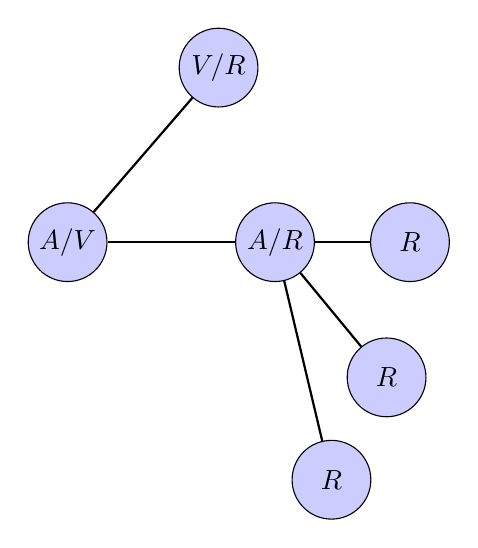
\begin{tikzpicture}
    \node[main node] (1) {$V/R$};
    \node[main node] (2) [below left = 1.5cm and 1.2cm of 1]  {$A/V$};
    \node[main node] (3) [below right = 1.5cm and 0.0cm of 1] {$A/R$};
    \node[main node] (4) [below right = 2.3cm and 0 cm of 3] {$R$};
    \node[main node] (5) [below right = 1cm and 0.7cm of 3] {$R$};
    \node[main node] (6) [right = 0.7cm  of 3] {$R$};

    \path[draw,thick]
    (1) edge node {} (2)
    (2) edge node {} (3)
    (3) edge node {} (4)
    (6) edge node {} (3)
    (5) edge node {} (3);
    %%
    
\end{tikzpicture}

\caption{NodosEstado de A y B.}
\end{center}

 si bien el grafo tiene un coloreo optimo donde 0=v 1=r 2=a 3...=r, El proceso por el que pasa nuestro algoritmo es el siguiente:
 \begin{enumerate}
 \item Si elijo verde cuantas posibilidades tengo? Los vecinos de 0 son 1 y 2 por ende: Posibilidades = #(colores(1)-verde)+#(colores(2)-verde) = 1+1=2
 \item Si elijo azul cuantas posibilidades tengo? Los vecinos de 0 son 1 y 2 por ende: Posibilidades = #(colores(1)-azul)+#(colores(2)-azul) = 1+2=3
 \item Elijo azul y avanzo hacia el nodo 1.
 \item El nodo 1 ahora solo tiene un color disponible que es el rojo, por ende lo seteo de tal manera y voy a sus vecinos.
 \item Todos los vecinos de 1 son unicamente de color rojo, por ende por cada vecino que tenga tal que solo puede ser pintado de rojo, el algoritmo encontrara un conflicto.
 \end{enumerate}\\

 
Nuestra hipotesis a analizar en los tests, es que para grafos generados pseudo-aleatoriamente y con una variedad amplia de colores, la segunda heuristica tiene mayor tiempo de ejecucion respecto de la primera ya que debe recorrer todos los colores del nodo para encontrar el que maximiza las posibilidades, pero encontrara un resultado mas cercano la optimo. Mientras menos dispersos esten los colores, mas cercanos creemos que seran los tiempos de ejcucion. \\

Una vez analizada la hipotesis, se nos ocurrio dessarrollar una tercer heuristica que es simplemente una variante de la recien mencionada:
Decidimos entonces desarrollar una heurisita que funcione igual que la segunda pero que recorra un determinado X$\div$ de los colores, siempre y cuando al llegar al X$\div$ haya encontrado un color valido. En caso de no encontrarlo, seguira iterando los colores hasta hacerlo. No sabemos que comportamiento tendra, pero nuestra hipotesis es que se situara en el medio de las otras dos, es decir que sera mejor que la primera y peor que la segunda a la hora de analizar la cantidad de conflictos pero a medida que ese porcentaje aumente, el tiempo de ejecucion aumentara tambien.

\subsection{Pseudo-C\'odigo}

\begin{verbatim}
solve()
FOREACH materias(grafo) as materia   // O(cantidad(Materias))
    IF cantidadColores(materia) == 1 THEN  // 
        colorFinal(materia) = color(materia);  // O(1)
    ELSE
    var Boolean seteeColor = false;            // O(1)
    int i; int color = 0;                     // O(1)
        FOR i desde 0 hasta cantidadColores(materia) Y !seteeColor   // O(cantidadColores(materia)
            boolean colorValido = true;
            color =  color(materia,i);
            FOREACH  vecinos(materia) as vecino                      // O(#vecinos(materia))
                IF noTieneColorFinal(vecino) THEN
                    IF (colores(vecino) != 1 && esta(color,colores(vecinos))){ // O(cantidadColores(materia)
                        colorValido = false;
                    ENDIF
                ELSE

                IF colorFinal(vecino) == color
                    colorValido = false;
                ENDIF

                IF colorValido 
                    seteeColor = true;
                    setearColorFinal(materia, color)
                ENDIF
            ENDFORECH
        ENDFOR
    IF ! seteeColor
        setearColorFinal(materia, color)   // O(1)
    ENDFOR
ENDFOREACH
\end{verbatim}

\subsection{Justificaci\'on y Complejidad}
\\
Como pudimos ver en la seccion anterior, podemos dar una analisis de complejidad en un peor caso, tomando cotas superiores en varios puntos del algoritmo.\\
Lo que podemos decir que es que para cada materia, haremos muchas operaciones de orden constante y un FOR que recorre todos los colores de la materia. Dentro de ese ciclo, volvemos a usar operaciones del orden constante y utilizamos otro clcio que involuchra todos los vecinos de la materia en cuestion.\\

Simplificando la complejidad del algoritmo, se observa que es un "Para todos las materias => Para Todos los colores de la materia => Para todos los vecinos de la materia => Operaciones O(1)" \\. La cantidad de colores de la materia esta acotado por la maxima cantidad de colores que tenga una materia, que por simplicidad llamaremos M. La cantidad de vecinos esta acotada tambien por la cantidad de materias en todo el grafo (ninguna materia puede tener mas vecinos que todas las materias del grafo), Por ende la complejidad viene dada por O(Cantmaterias*M*CantMaterias)\subset O(Cantmaterias^2 * M)


\subsection{Tests y Performance}

En esta seccion vamos a realizar distintas pruebas:
\begin{enumerate}
 \item Para un grafo que sepamos que funciona mal en la H1, veremos su funcionamiento en H2 en relacion a la cantidad de conflictos.
 \item Para un grafo que sepamos que funciona mal en la H2, veremos su funcionamiento en H1 en relacion a la cantidad de conflictos.
 \item Analizaremos como se comporta un grafo aleatorio en relacion a los conflictos para H1 y H2 y los tiempos de ejecucion.
 \item Una vez comparadas las heuristicas H1 y H2, veremos como funciona el tema conflcitos y los tiempos de ejecucion en la H3 con distitntas variantes:
 \begin{enumerate}
 \end{enumerate}\\
 
Por otro lado veremos como crece la complejidad y la cantidad de conflicos del problema al aumentar la cantidad de aristas para cada una de nuestras heuristicas. \\
\begin{figure}[h!]
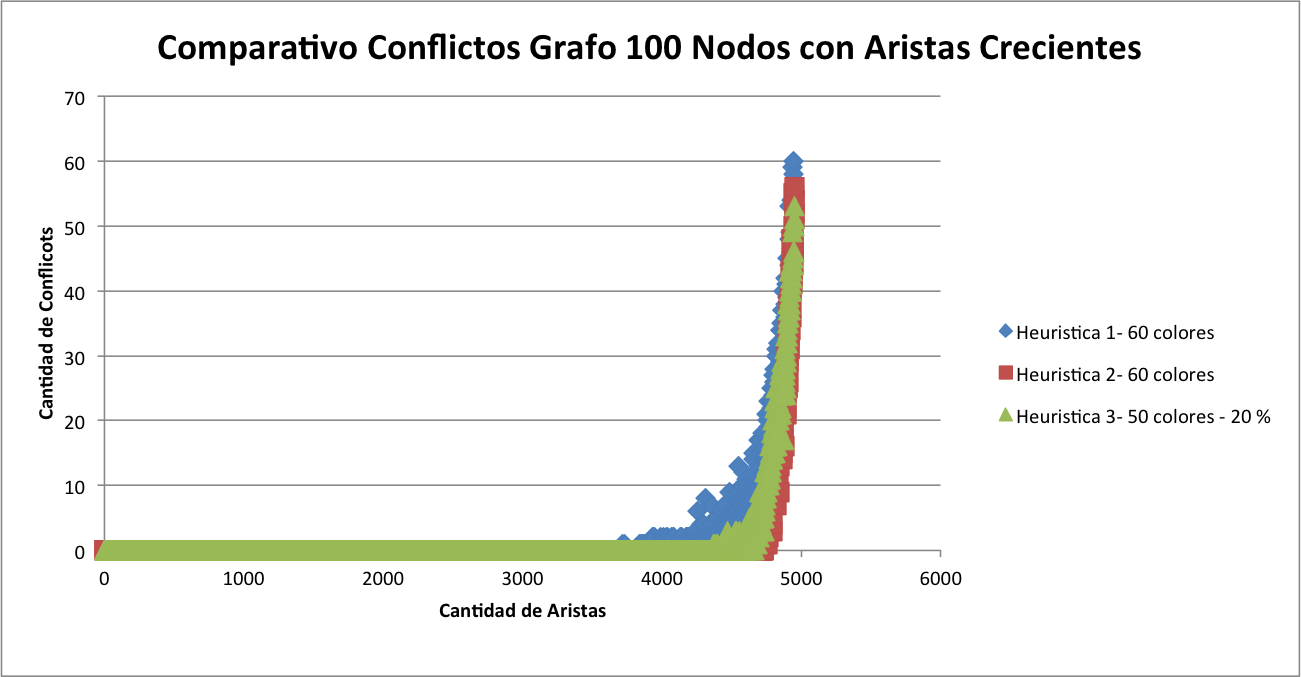
\includegraphics[width=140mm]{ejercicio3/ej3-comparativo-grafo100-conflicto.png}
\centering
\caption{comparativa conflictos aumento de aristas}
\label{overflow3}
\end{figure}
 \pagebreak
\\ 
\begin{figure}[h!]
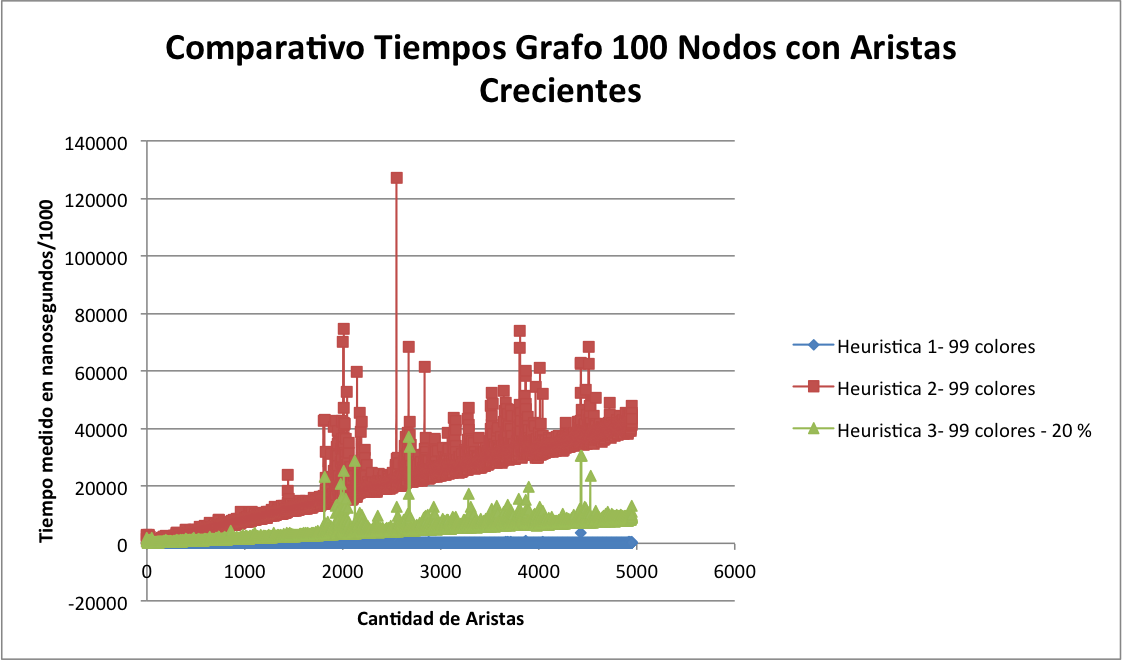
\includegraphics[width=140mm]{ejercicio3/ej3-comparativo-grafo100-tiempo-99colores.png}
\centering
\caption{comparativa tiempos aumento de aristas 100 colores}
\label{overflow3}
\end{figure}
\\

\begin{figure}[h!]
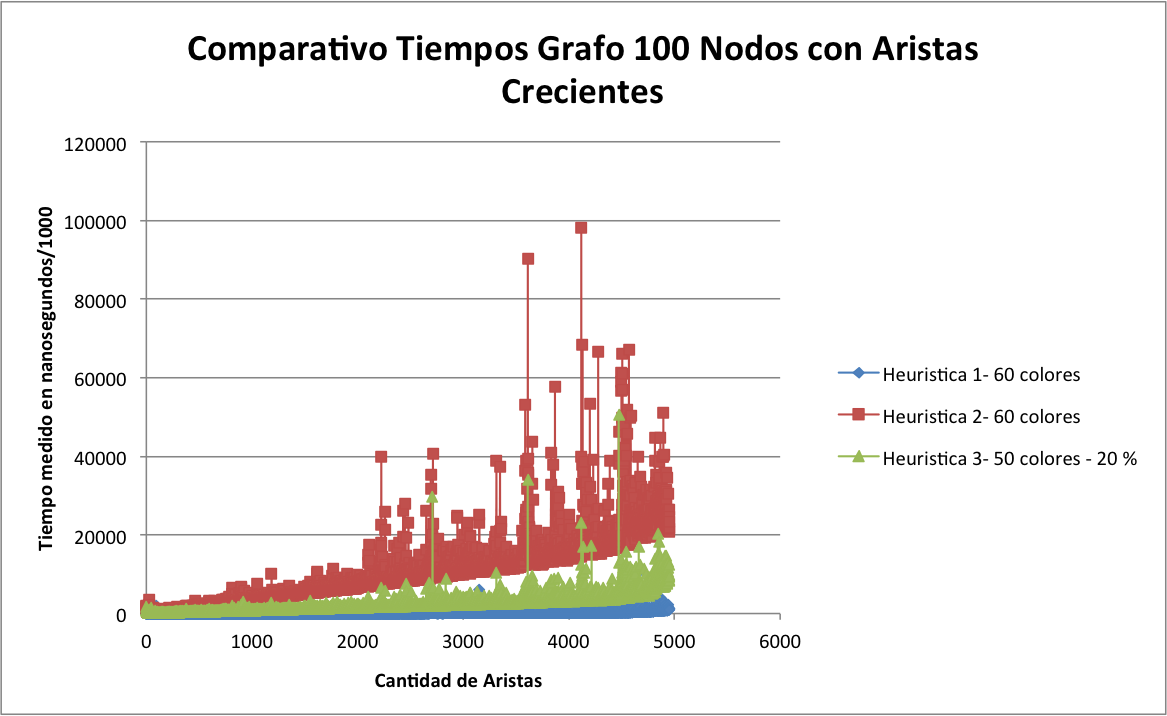
\includegraphics[width=140mm]{ejercicio3/ej3-comparativo-grafo100-tiempo.png}
\centering
\caption{comparativa tiempo aumento de aristas 50 colores}
\label{overflow3}
\end{figure}
\\
\pagebreak
\newpage
\begin{figure}[h!]
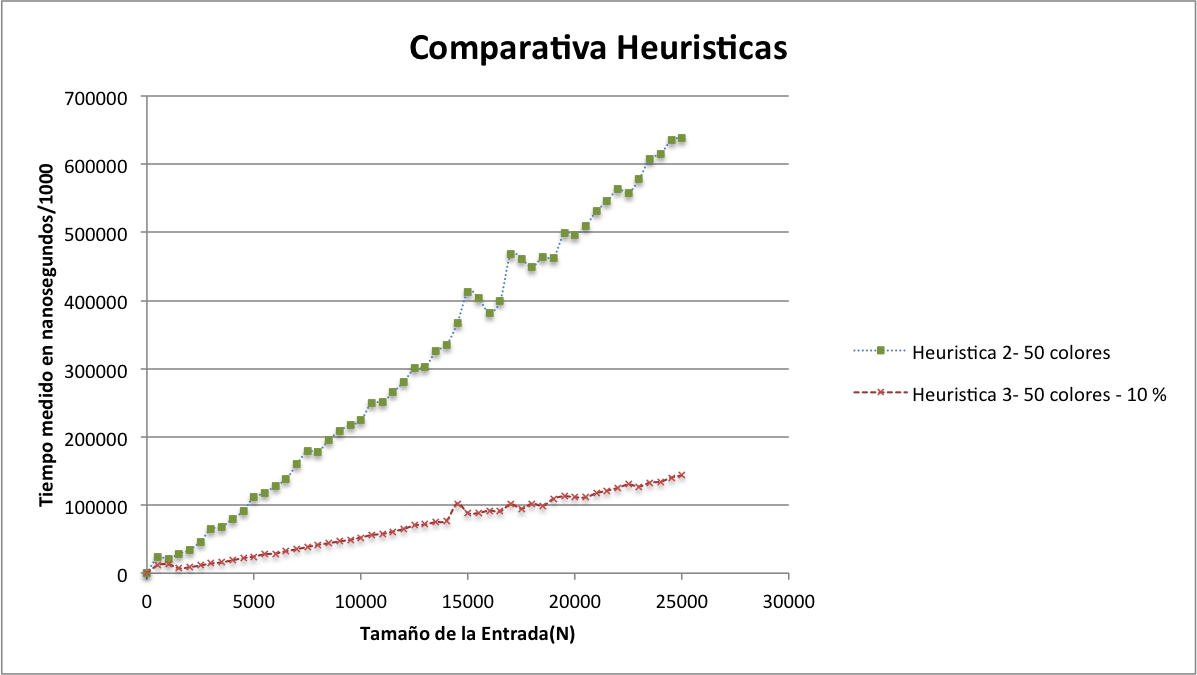
\includegraphics[width=140mm]{ejercicio3/ej3-comparativo-10.png}
\centering
\caption{Comparacion tiempo h2 Vs tiempo h3 10}
\label{overflow3}
\end{figure}



Lo que podemos apreciar es que la complejidad del algoritmo depende primordialmente de la cantidad de aristas ya que esta modifica la cantidad de vecinos de cada nodo. Esto sucede por que en el algoritmo vemos que la mayoria de cuentas se producen dentro del ciclo que reocrre los vecinos. Para un nodo que no tiene vecinos, simplente seteamos un color, mientras que por cada vecino tendremos que chequear varias cosas que si bien son O(1), suman.\\
Ahora analizaremos lo antes mencionado. \\
1 y 2)\\ Mediante la siguiente tabla podemos ver que encontramos una familia de grafos y de distribuciones de colores tal que si bien tienen coloreos validos, nuestras heuristicas los rompen tanto como quieran.\\
\begin{tabular}{| l | c | r |}
  \hline
Grafo Solucion Optima Al Final  & GrafoRompe Heuristica 2 & Aleatorio 100 nodos \\ \hline
6  & 0 & 169\\ \hline
1  & 10 & 92\\ \hline
\end{tabular}

\\Para la primer heuristica, si para cada nodo, el color que corresponde al coloreo valido se encuentra en el ultimo lugar, primero revisara todos los anteriorir y en caso de encontrar uno que localmente sirva, no llegara a revisar el color optimo y lo perdera.\\
Por otro lado, como mencionamos en la explicacion, la heuristica dos puede funcionar infinitamente mal (ver ejemplo).\\
Ademas vemos que para un grafo aleatorio de 100 nodos y relativamente denso, la heuristica dos es un poco mas eficiente que la uno en cuanto a cantidad de conflictos.

3) Veamos que si todos los nodos tienen un solo color, las heuristicas tardaran lo mismo ya que la segunda heuristica no debe recorrer todos los colores del nodo (tiene uno solo).\\

\begin{figure}[h!]
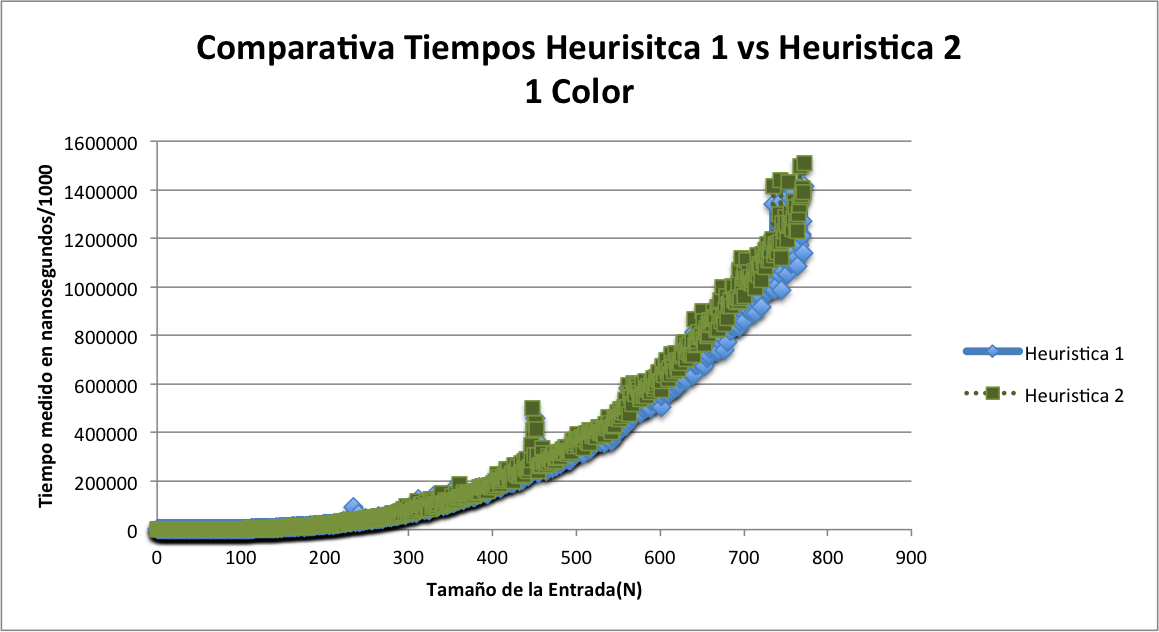
\includegraphics[width=140mm]{ejercicio3/ej3-comparativo-eu1-eu2-grafoCreciente-tiempo-1color.png}
\centering
\caption{Comparacion tiempo h1 Vs tiempo h2 1 color por nodo}
\label{overflow3}
\end{figure}


Ahora veamos que sucede si le ponemos N colores:\\

\pagebreak
\begin{figure}[h!]
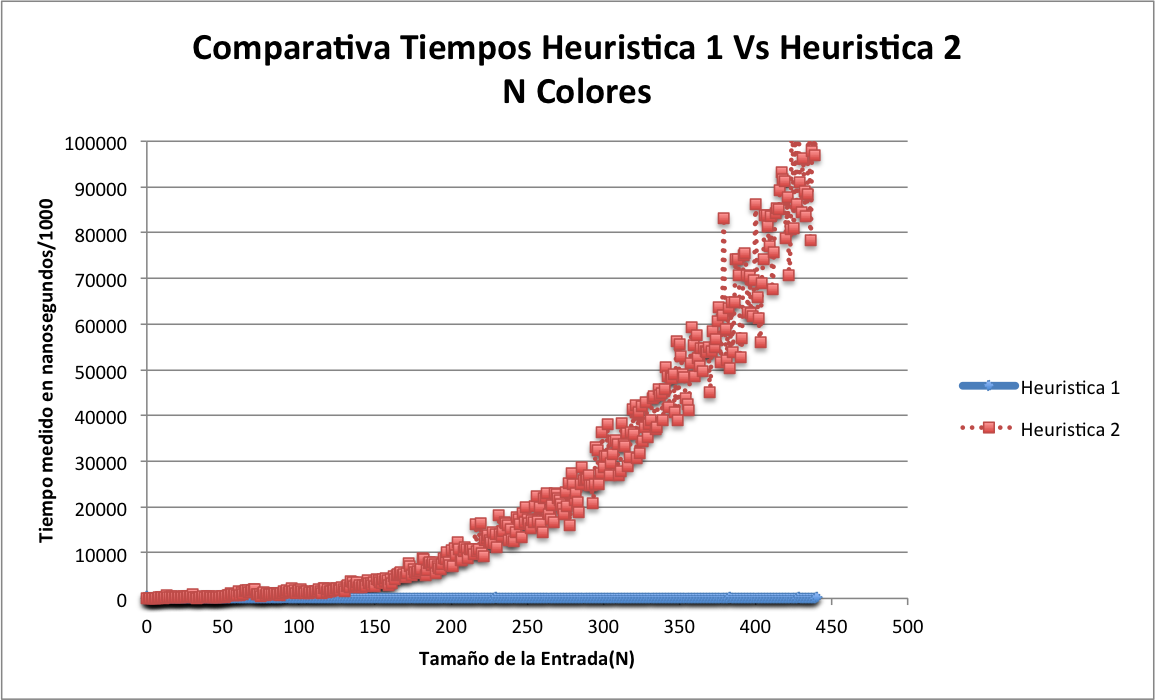
\includegraphics[width=140mm]{ejercicio3/ej3-comparativo-eu1-eu2-grafoCreciente-tiempo.png}
\centering
\caption{Comparacion tiempo h1 Vs tiempo h2 N colores por nodo}
\label{overflow3}
\end{figure}

La conclusion que sacamos es que al tener muchos colores, la H1 encontrara un color valido en algun momento y no llegara a revisar toda la lista de colores por completo como si lo hace la H2. Con respecto a los conflictos, el analisis esta plasmado en el cuadro de 1 y 2.\\
4) Antes de empezar decidimos no utilizar la H3 10porciento para los grafos con 10 colores ya que carece de sentido. Tambien aclararemos que el grafo utilizado es un grafo de 25k nodos no tan denso.\\


\begin{figure}[h!]
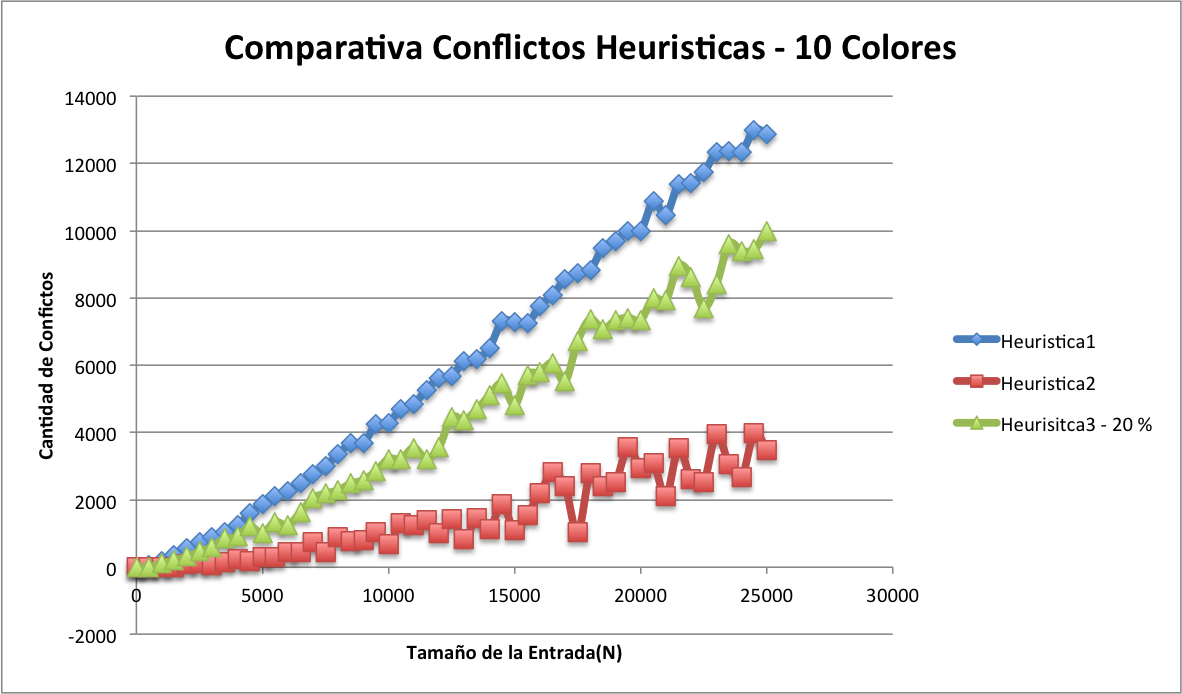
\includegraphics[width=140mm]{ejercicio3/ej4-comparativa-conflictos-10.png}
\centering
\caption{Comparacion conflictos h1 vs h2 Vs h3 10 colores por nodo}
\label{overflow3}
\end{figure}

\pagebreak

\begin{figure}[h!]
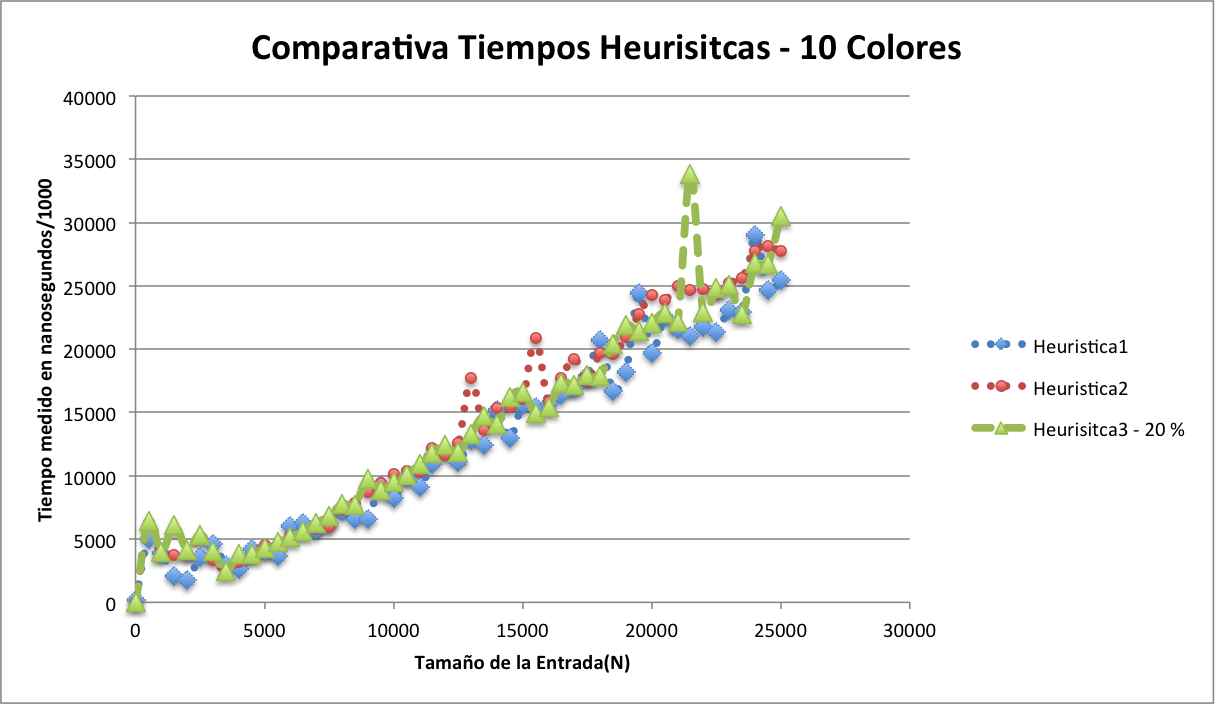
\includegraphics[width=140mm]{ejercicio3/ej4-comparativa-tiempos-10.png}
\centering
\caption{Comparacion tiempos h1 vs h2 Vs h3 10 colores por nodo}
\label{overflow3}
\end{figure}
\\
\\
Lo que podemos apreciar en los anteriores graficos es que cuando tenemos pocos colores, el tiempo de ejecucion es similiar para las tres heuristicas. Como estamos en un grafo de muchos nodos, es muy probable que con 10 colores, siempre encuentres un conflicto, por lo que la H1, tendera a revisar muchos colores. La H2, revisa todos los colores siempre y por otro lado la h3 solo revisa un porcentaje pero ya que sucede lo mismo que con la H1, tiende a revisar la mayoria de los colores. En relacion a los conflictos, vemos que la H2 es la que mejor se comporta ya que siempre que localmente haya un color valido, lo seteara mientras que la H1 se quedara con el primero que encuentre que sea valido.\\
\\
\\
\begin{figure}[h!]
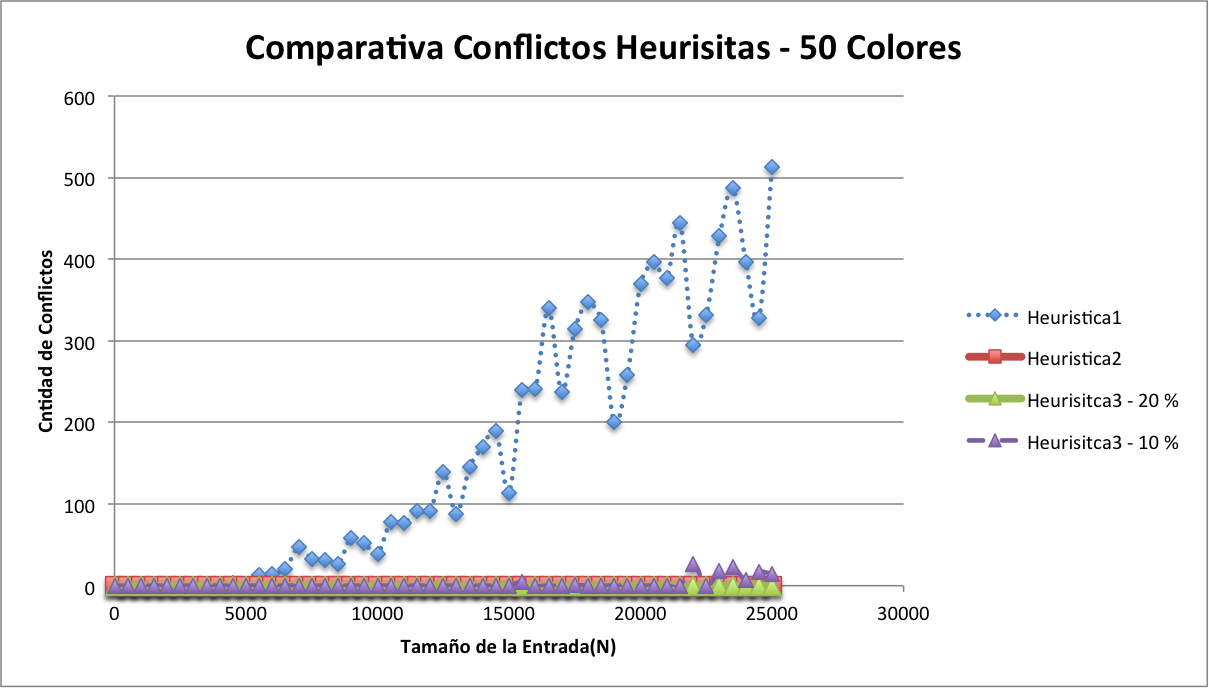
\includegraphics[width=140mm]{ejercicio3/ej4-comparativa-conflictos-50.png}
\centering
\caption{Comparacion conflictos h1 vs h2 Vs h3 50 colores por nodo}
\label{overflow3}
\end{figure}
\\
\\
\begin{figure}[h!]
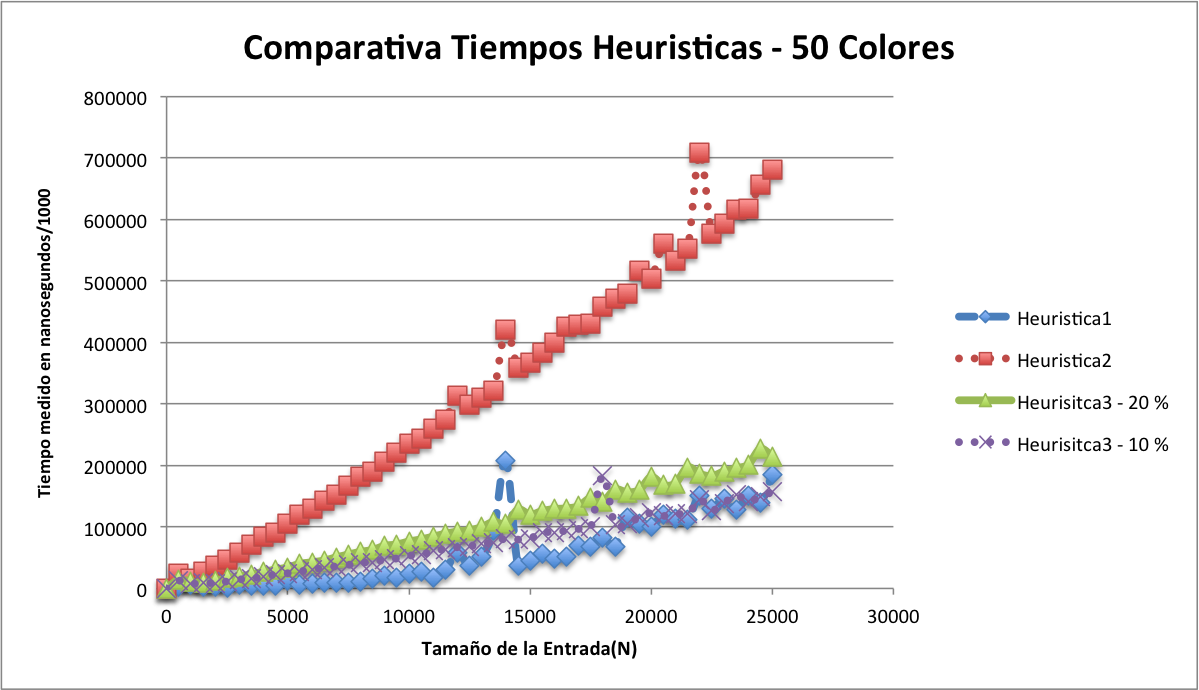
\includegraphics[width=140mm]{ejercicio3/ej4-comparativa-tiempos-50.png}
\centering
\caption{Comparacion tiempos h1 vs h2 Vs h3 50 colores por nodo}
\label{overflow3}
\end{figure}

\pagebreak
Si tenemos muchos colores ( Hicimos el analisis para 50 colores y 0,5$\%$ de densidad) la H2 debera recorrerlos todos y eso hara demasiada diferencia ante la H1 donde recorrera unicamente hasta encontrar un color valido. Paliativamente tenemos la H3 que como muy bien indica el grafico, mientras mas alto sea el porcentaje de colores a revisar, mas tiempo tardara en hallar la solucion.\\
A la hora de analizar el tema de los conflictos, al igual que antes la H1 no funiona muy bien ya que nos encuentra muchisimos conflictos. Sin embargo vemos como las demas heuristicas si bien han pagado un tiempo de ejecucion mayor, nos encontraron coloreos validos.
\pagebreak